\documentclass[a4paper]{tufte-handout}

\usepackage{/Users/paulallen/OU/Maths/style}

\begin{document}
\tma{03}

%%%%%%%%%%Question one
\begin{question}

\qpart

\marginnote{
Product rule, for
\begin{align*}
  f(x) &= g(x)h(x)\\
  f^{\prime}(x) &= g(x)h^{\prime}(x) + h(x)g^{\prime}(x)
\end{align*}}

\begin{align*}
  f(x) &= (x^{5} + 3x^{3} + 2x + 1)e^{x}\\[8pt]
  \stext{Using}
  g &= x^{5} + 3x^{3} + 2x + 1\\[8pt]
  \stext{and}
  h &= e^{x}\\[8pt]
  \stext{Differentiating}
  g^{\prime} &= 5x^{4} + 9x^{2} + 2\\[8pt]
  \stext{and}
  h^{\prime} &= e^{x}\\[8pt]
  \stext{Using the product rule}
  f^{\prime}(x) &= (5x^{4} + 9x^{2} + 2)e^{x} + e^{x}(x^{5} + 3x^{3} + 2x + 1)\\[8pt]
  \stext{Simplifying}
  &= (x^{5} + 5x^{4} + 3x^{3} + 9x^{2} + 2x + 3)e^{x}
\end{align*}

\vspace{5cm}

\qpart

\marginnote{
Chain rule, for
\begin{align*}
  g(y) &= i(h(y))\\[8pt]
  g^{\prime}(y) &= i^{\prime}(h(y))h^{\prime}(y)
\end{align*}}

\begin{align*}
  g(y) &= \rb{\ln{(y)} + \sin{(y)}}^{6}\\[8pt]
  \stext{Using}
  h(y) &= \ln{(y)} + \sin{(y)}\\[8pt]
  \stext{and}
  i(h) &= h^{6}\\[8pt]
  \stext{Differentiating}
  h^{\prime}(y) &= \rb{\frac{1}{y} + \cos{y}}\\[8pt]
  \stext{and}
  i^{\prime}(h) &= 6h^{5}\\[8pt]
  \stext{Using the chain rule}
  g^{\prime}(y) &= 6\sqb{\ln{(y)} + \sin{(y)}}^{5}\rb{\frac{1}{y} + \cos{(y)}}
\end{align*}

\vspace{5cm}

\qpart

\marginnote{
Quotient rule, for
\begin{align*}
  h(z) &= \frac{i(z)}{j(z)}\\
  h^{\prime}(z) &= \frac{j(z)i^{\prime}(z) - i(z)j^{\prime}(z)}{(j(z))^{2}}
\end{align*}}

\begin{align*}
  h(z) &= \frac{e^{5z}}{(2 + \cos{(10z)})}\\[8pt]
  \stext{Using}
  i(z) &= e^{5z}\\[8pt]
  \stext{and}
  j(z) &= (2 + \cos(10z))\\[8pt]
  \stext{Differentiating}
  i^{\prime}(z) &= 5e^{5z}\\[8pt]
  \stext{and}
  j^{\prime}(z) &= -10\sin(10z)\\[8pt]
  \stext{Using the quotient rule}
  h^{\prime}(z) &= \frac{(2 + \cos{(10z)})5e^{5z} - e^{5z}\rb{-10\sin{(10z)}}}{\rb{2 + \cos{(10z)}}^{2}}\\[8pt]
  \stext{Simplifying}
  &= \frac{5e^{5z}\rb{(2 + \cos{(10z)}) + \rb{2\sin{(10z)}}}}{(2 + \cos{(10z)})^{2}}
\end{align*}

\vspace{5cm}

\qpart

\marginnote{
\begin{align*}
  \stext{Product rule: }
  k(x) &= l(x)m(x)\\[8pt]
  k^{\prime}(x) &= l(x)m^{\prime}(x) + l^{\prime}(x)m(x)\\[8pt]
  \stext{Chain rule}
  m^{\prime}(x) &= u^{\prime}(v(x))v^{\prime}(x)
\end{align*}
}

\begin{align*}
  k(x) &= x^{2}\sin{(\cos{x})} \\[8pt]
  \stext{Using}\\
  & l(x) = x^{2} \quad \text{and} \quad m(x) = \sin{(\cos{x})} \\[8pt]
  \stext{Differentiating using the product rule}\\
  & l^{\prime}(x) = 2x \\[8pt]
  \stext{Now using the chain rule to find \( m^{\prime}(x) \), using \( u = \sin{(x)} \) and \( v = \cos{(x)} \)}\\
  u^{\prime} &= \cos{(x)}\\[8pt]
  \stext{and}\\
  v^{\prime} &= -\sin{(x)}\\[8pt]
  \stext{Thus}\\
  m^{\prime} &= \cos(\cos{x})\rb{-\sin(x)}\\[8pt]
  \stext{Applying the product rule}\\
  k^{\prime}(x) &= x^{2}(\cos(\cos{x})\rb{-\sin(x)}) + 2x\sin{(\cos{x})} \\[8pt]
  \stext{Simplifying}\\
  &= 2x\sin(\cos{x}) -x^{2}\sin(x)\cos(\cos{x})
\end{align*}

\end{question}

\clearpage
%%%Question two

\begin{question}

Given the L-shaped enclosure

\begin{center}
	\begin{tikzpicture}
		\tkzDefPoint(-2,0){a}
		\tkzDefPoint(4,0){b}
		\tkzDefPoint(4,2){c}
		\tkzDefPoint(0,2){d}
		\tkzDefPoint(0,4){e}
		\tkzDefPoint(-2,4){f}
		\tkzDrawSegments(a,b b,c c,d d,e e,f f,a)
		\tkzLabelSegment[below](a,b){$x+5$}
		\tkzLabelSegment[right](b,c){$y$}
		\tkzLabelSegment[above](c,d){$5$}
		\tkzLabelSegment[right](d,e){$y$}
		\tkzLabelSegment[above](e,f){$x$}
		\tkzLabelSegment[left](f,a){$2y$}
	\end{tikzpicture}
\end{center}

\qpart

\begin{align*}
  \stext{Using the assumption that Steven uses all the fencing he has exactly the perimeter is \( \SI{74}{\metre} \)}
  perimeter &= \rb{x + 5} + y + 5 + y + x + 2y\\[8pt]
  74 &= 4y + 2x + 10\\[8pt]
  64 &= 4y + 2x\\[8pt]
  4y &= 64 - 2x\\[8pt]
  y &= 16 - \frac{x}{2}\\[8pt]
  &= \frac{1}{2}\rb{32 - x}\\[8pt]
  \snote{as required}
\end{align*}

\vspace{5cm}

\qpart

\begin{center}
	\begin{tikzpicture}
		\tkzDefPoint(-2,0){a}
		\tkzDefPoint(4,0){b}
		\tkzDefPoint(4,2){c}
		\tkzDefPoint(0,2){d}
		\tkzDefPoint(0,4){e}
		\tkzDefPoint(-2,4){f}
		\tkzDefPoint(0,0){g}
		\tkzDrawSegments(a,b b,c c,d d,e e,f f,a e,g)
		\tkzLabelSegment[right](b,c){$y$}
		\tkzLabelSegment[above](c,d){$5$}
		\tkzLabelSegment[above](e,f){$x$}
		\tkzLabelSegment[left](f,a){$2y$}
	\end{tikzpicture}
\end{center}

The area of the L-shape is given by the total of the two shapes shown above.

\begin{align*}
  A &= x\rb{2y} + 5\rb{y}\\[8pt]
  &= x\rb{2\rb{\frac{1}{2}\rb{32 - x}}} + 5\rb{\frac{1}{2}\rb{32 - x}}\\[8pt]
  &= x\rb{32 - x} + \rb{80 - \frac{5x}{2}}\\[8pt]
  &= 32x -x^{2} + 80 - \frac{5x}{2}\\[8pt]
\stext{Multiply by \( 2 \)}
  2A &= 160 + 64x - 5x -2x^{2}\\[8pt]
\stext{Collect like terms}
  &= 160 + 59x -2x^{2}\\[8pt]
\stext{simplify}
  A &= \frac{1}{2}\rb{160 + 59x -2x^{2}}\\[8pt]
  \snote{as required} 
\end{align*}

\vspace{5cm}

\qpart

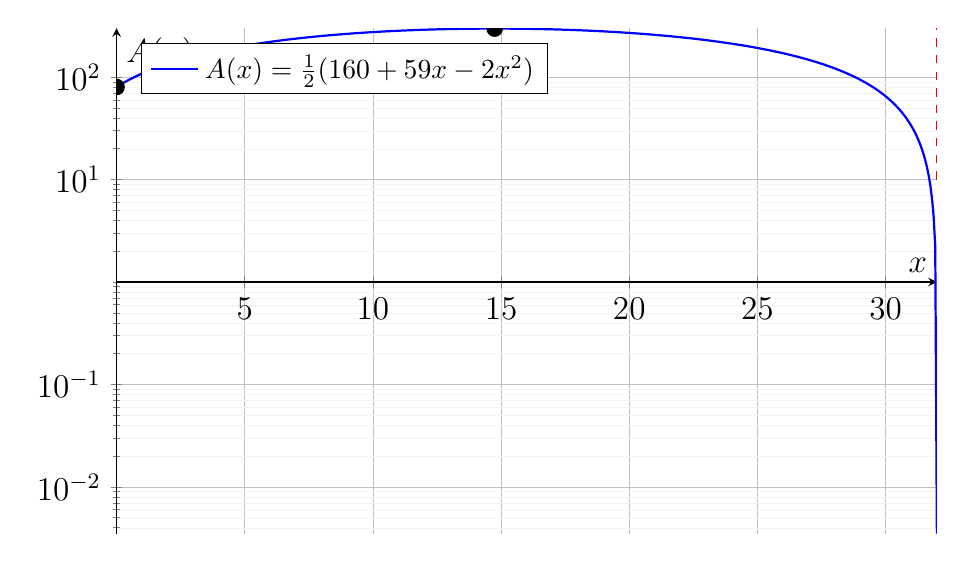
\begin{tikzpicture}
    \begin{axis}[
        width=12cm,
        height=8cm,
        xlabel={$x$},
        ylabel={$A(x)$},
        ymode=log,
        log basis y={10},
        ymin=0, ymax=300,
        xmin=0, xmax=32,
        domain=0:32,
        samples=500,
        grid=both,
        grid style={line width=.1pt, draw=gray!10},
        major grid style={line width=.2pt,draw=gray!50},
        axis lines=middle,
        legend pos=north west,
        xlabel style={font=\large},
        ylabel style={font=\large},
        tick label style={font=\large},
    ]
    \addplot [blue, thick] {0.5*(160 +59*x -2*x^2)};
    \addlegendentry{$A(x) = \frac{1}{2}(160 + 59x -2x^{2})$}
    
    % Mark the vertex
    \fill (14.75,297.56) circle (3pt) node[above right] {Vertex};
    
    % Mark the y-intercept
    \fill (0,80) circle (3pt) node[above left] {$(0,80)$};
    
    % Mark the asymptote at x=32
    \draw[dashed, red] (32,10) -- (32,300) node[above] {Asymptote at $x=32$};
    \end{axis}
\end{tikzpicture}

Based on the shape of the curve for this graph we need only consider the stationary point at which \( dA/dx = 0 \) to find the maximum area.

\begin{align*}
  \stext{Given}
  A &= \frac{1}{2}\rb{160 + 59x -2x^{2}}\\[8pt]
  \stext{Differentiating}
  A^{\prime} &= -2x + \frac{59}{2}\\[8pt]
  \stext{Setting \( A^{\prime} = 0 \) to find the stationary point}
  0 &= -2x + \frac{59}{2}\\[8pt]
  2x &=  \frac{59}{2}\\[8pt]
  x &=  \frac{59}{4}\\[8pt]
  \stext{Substituting this into the original equation}
  A &= \frac{1}{2}\rb{160 + 59x -2x^{2}}\\[8pt]
  &= \frac{1}{2}\rb{160 + 59\rb{\frac{59}{4}} -2\rb{\frac{59}{4}}^{2}}\\[8pt]
  &= 80 + \frac{3481}{8} - \rb{\frac{59}{4}}^{2}\\[8pt]
  &= 80 + \frac{3481}{8} - \rb{\frac{3481}{16}}\\[8pt]
  &= \frac{1280}{16} + \frac{6962}{16} - \rb{\frac{3481}{16}}\\[8pt]
  &= \frac{1280}{16} + \frac{3481}{16}\\[8pt]
  &= \frac{4761}{16}\\[8pt]
  \stext{Applying the second derivative test}
  A^{\prime} &= -2x + \frac{59}{2}\\[8pt]
  A^{\prime\prime} &= -2\\[8pt]
  \stext{Showing that this a maximum stationary point}
\end{align*}

Hence the maximum area of the L-shape is 
  \[ A = \frac{4761}{16}\unit{\metre\squared} \]

\end{question}

\clearpage
%%%Question three

\begin{question}

\qpart

\begin{align*}
  f(x) &= x^{2} + 2x + 5\\[8pt]
  \stext{Then the indefinite integral is}
  F(x) & = \frac{x^{3}}{3} + x^{2} + 5x + c\\[8pt]
\end{align*}

\vspace{2cm}

\qpart

\begin{align*}
  g(\theta) &= 5e^{\theta} + \frac{1}{5\theta}\\[8pt]
  \stext{Then the indefinite intergral is}
  G(\theta) & = 5e^{\theta} + \frac{\ln{\theta}}{5} + c\\[8pt]
\end{align*}

\vspace{2cm}

\qpart

\begin{align*}
  h(t) &= 2\sin{(t)} + \frac{1}{3 + 3t^{2}} + 3\\[8pt]
  &= 2\rb{\int\sin{(t)}}dt + \frac{1}{3}\rb{\int{\frac{1}{1 + t^{2}}}}dt + 3\\[8pt]
  \stext{Then the indefinite intergral is}
  H(t) & = -2\cos{(t) + \frac{1}{3}\taninv{(t)}} + 3t + c\\[8pt]
  &= \frac{1}{3}\rb{\taninv{(t)} - 6\cos{(t)} + 9t + c }
\end{align*}

\clearpage

\qpart

\begin{align*}
  j(y) &= \rb{y - 2}\rb{y^{\frac{-1}{2}}} + 3)\\[8pt]
  \stext{Expand the brackets}
  &= y^{\frac{1}{2}} + 3y - 2y^{\frac{-1}{2}} - 6\\[8pt]
  &= y^{\frac{1}{2}} + \rb{3\int{y}}dy - \rb{2\int{y^{\frac{-1}{2}}}}dy - 6\\[8pt]
  \stext{Then the indefinite intergral is}
  J(y) & = \frac{1}{\frac{3}{2}}y^{\frac{3}{2}} + 3\rb{\frac{1}{2}y^{2}} -2\rb{\frac{1}{\frac{1}{2}}y^{\frac{1}{2}}} - 6y + c\\[8pt]
  &= \frac{2t^{\frac{3}{2}}}{3} + \frac{3y^{2}}{2} - 4\sqrt{y} - 6y + c
\end{align*}

\end{question}

\clearpage

%%%Question four

\begin{question}

  \[ f(x) = -x^{2} + 4x +12 \]

\qpart

As the function is an inverted U parabola the x-intersection points will show were the curve crosses to below the x-axis.

\begin{align*}
  f(x) &= -x^{2} + 4x + 12\\[8pt]
  \stext{Substituting both \( -2 \) and \( 6 \) into the equation}
  f(-2) &= -(-2)^{2} + 4(-2) + 12\\[8pt]
  &= -4 - 8 + 12\\[8pt]
  &= 0\\[8pt]
  \stext{and}
  f(6) &= -(6)^{2} + 4(6) + 12\\[8pt]
  &= -36 + 24 + 12\\[8pt]
  &= 0
\end{align*}

Hence the graph between and not including these points are above the x-axis.

\vspace{3cm}

\qpart

\begin{align*}
  f(x) &= -x^{2} + 4x + 12\\[8pt]
  &= \int_{1}^{3} \rb{-x^{2} + 4x + 12}\dif{x}\\[8pt]
  &= \rb{-\int{x^{2}} + 4\int{x} + 12 \int{1}}\dif{x}\\[8pt]
  &= \rb{\frac{-1}{3}x^{3} + 4\rb{\frac{1}{2}x^{2}} + 12(x)}\\[8pt]
  &= \sqb{\frac{-1}{3}x^{3} + 8x^{2} + 12x}_{1}^{3}\\[8pt]
\end{align*}

\qpart

Using this to find the area under the curve between \( -2 < x < 6 \)

\begin{align*}
  f(x) &= -x^{2} + 4x + 12\\[8pt]
  &= \int_{-2}^{6} \rb{-x^{2} + 4x + 12}\dif{x}\\[8pt]
  &= \sqb{\frac{-1}{3}x^{3} + 4\rb{\frac{1}{2}}x^2 + 12x}_{-2}^{6}\\[8pt]
  &= \rb{\frac{-1}{3}6^{3} + 2\rb{6}^{2} + 12\rb{6}} - \rb{{\frac{-1}{3}\rb{-2}^{3} + 2\rb{-2}^{2} + 12\rb{-2})}}\\[8pt]
  &= \rb{\frac{-1}{3}\rb{216} + \rb{2}36 + 72} - \rb{\frac{-1}{3}\rb{-8} + \rb{2}4 - 24}\\[8pt]
  &= \rb{-72 + 72 + 72} - \rb{\frac{8}{3} + 8 - 24}\\[8pt]
  &= 72 - \rb{\frac{-40}{3}}\\[8pt]
  \stext{Hence the area under the curve between \( x=-2 \) and \( x=6 \) is}\\[8pt]
&=  \frac{256}{3}
\end{align*}

\end{question}

\clearpage

%%%Question five

\begin{question}

\qpart

	\[ \int{\frac{\cos\rb{3x} - \sin\rb{3x}}{\rb{\sin\rb{3x} + \cos\rb{3x}}^2}} \]

  \begin{align*}
    \stext{substitute \( u=3x \) and \( \dif{u}=3\dif{x} \)}\\[8pt]
    &= \frac{1}{3}\int{\frac{\cos\rb{u} - \sin\rb{u}}{\rb{\sin\rb{u} + \cos\rb{u}}^2}}\dif{u}\\[8pt]
    \stext{Substitute \( v= \sin\rb{u} + \cos\rb{u}, \dif{v}= \cos\rb{u} - \sin\rb{u}\dif{u} \)}\\[8pt]
    &= \frac{1}{3}\int{\frac{1}{v^{2}}\dif{v}}\\[8pt]
    &= \frac{1}{3}\rb{-\frac{1}{v}} + C\\[8pt]
    \stext{Substituting \( v \) back in}\\[8pt]
    &= \frac{-1}{3\rb{\sin{u} + \cos{u}}} + C\\[8pt]
    \stext{Substituting \( u \) back in}\\[8pt]
    &= \frac{-1}{3\rb{\sin{3x} + \cos{3x}}} + C
  \end{align*}

\clearpage

\qpart

   \[ \int_{0}^{\frac{1}{3}\ln{5}} e^{3x}\sqrt{e^{3x}+2} \dif{x} \]

   \begin{align*}
    &\stext{Substitute \( u = 3x \), \( \dif{u} = 3 \dif{x} \)}\\[8pt]
    &= \frac{1}{3} \int_{0}^{\ln{5}} e^{u} \sqrt{e^{u} + 2} \dif{u}\\[8pt]
    &\stext{Substitute \( v = e^{u} + 2 \), \( \dif{v} = e^{u} \dif{u} \)}\\[8pt]
    &= \frac{1}{3} \int_{0}^{\ln{5}} \sqrt{v} \dif{v}\\[8pt]
    &\stext{The integrand of \( v \) is \(\frac{2}{3} v^{\frac{3}{2}}\)}\\[8pt]
    &= \frac{1}{3} \rb{\frac{2}{3} v^{\frac{3}{2}}}\\[8pt]
    &= \frac{2}{9} v^{\frac{3}{2}}\\[8pt]
    &\stext{Substitute \( v \) back in}\\[8pt]
    &= \frac{2}{9} \rb{e^{u} + 2}^{\frac{3}{2}}\\[8pt]
    &\stext{Substitute \( u \) back in}\\[8pt]
    &= \frac{2}{9} \rb{e^{3x} + 2}^{\frac{3}{2}}
\end{align*}

It follows that

\begin{align*}
  \int_{0}^{\frac{1}{3}\ln{5}} e^{3x}\sqrt{e^{3x}+2} \dif{x} &= \sqb{\frac{2}{9} \rb{e^{3x} + 2}^{\frac{3}{2}}}_{0}^{\frac{1}{3}\ln{5}}\\[8pt]
  &= \sqb{\frac{2}{9} \rb{e^{3\rb{\frac{1}{3}\ln{5}}} + 2}^{\frac{3}{2}}} - \sqb{\frac{2}{9} \rb{e^{3\rb{0}} + 2}^{\frac{3}{2}}}\\[8pt]
  &= \sqb{\frac{2}{9} \rb{5 + 2}^{\frac{3}{2}}} - \sqb{\frac{2}{9} \rb{1 + 2}^{\frac{3}{2}}}\\[8pt]
  &= 4.115\ldots - 1.154\ldots\\[8pt]
  &= 2.96\\[8pt]
  \snote{to 2 d.p}
\end{align*}

\end{question}

%%%Question six

\begin{question}
  
\marginnote{Integration py parts \[ \int{f(x)g(x)\dif{x}} = f(x)G(x)-\int{f^{\prime}G(x)}\dif(x) \]}

\qpart

\begin{align*}
  \int{81x^{8}\ln{(x)}\dif{x}}\\[8pt]
\stext{Let, \( f(x)=\ln((x)) \) and \( g(x)=x^{8} \)}\\[8pt]
\stext{Then, \( f^{\prime}(x)=\frac{1}{x} \) and \( G(x)=\frac{x^{9}}{9} \)}\\[8pt]
  &= 81\int{x^{8}\ln{(x)}\dif{x}}\\[8pt]
  &= 81\sqb{\ln{(x)}\frac{x^{9}}{9} - \int(\frac{x^{9}}{9x})\dif{x}}\\[8pt]
  &= 9\rb{\ln((x))x^{9} - \int{x^{8}}\dif{x}}\\[8pt]
  &= 9\rb{\ln{(x)}x^{9} - \frac{x^{9}}{9}}\\[8pt]
  &= 9\ln{(x)}x^{9} - x^{9}\\[8pt]
  &= 9x^{9}\rb{\ln{(x)} - 1}
\end{align*}

\vspace{5cm}
\qpart

\begin{align*}
  \int{e^{3y}\sin{(2y)}\dif{y}} &=\\[8pt]
\stext{Let, \( f(y)=\sin(2y) \) and \( g(y)=e^{3y} \)}\\[8pt]
\stext{Then, \( f^{\prime}(y)=2\cos(2y) \) and \( G(y)=\frac{e^{3y}}{3} \)}\\[8pt]
  &= \frac{1}{3}e^{3y}\sin{2y} - \frac{2}{3}\int{e^{3y}\cos(2y)\dif{y}}\\[8pt]
\stext{Let, \( h(y)=\cos(2y) \) and \( i(y)=e^{3y} \)}\\[8pt]
\stext{Then, \( h^{\prime}(y)=-2\sin(2y) \) and \( I(y)=\frac{e^{3y}}{3} \)}\\[8pt]
  &= \frac{1}{3}e^{3y}\sin{2y} - \frac{2}{3}\sqb{\frac{e^{3y}\cos(2y)}{3} - \frac{2}{3}\int{e^{3y}\sin(2y)\dif{y}}}\\[8pt]
  &= \frac{1}{3}e^{3y}\sin(2y) - \frac{2}{9}e^{3y}\cos(2y) - \frac{4}{9}\int{e^{3y}\sin(2y)\dif{y}}\\[8pt]
\stext{Add \( \frac{4}{9}\int{e^{3y}\sin(2y)}\dif{y} \) to both sides}\\[8pt]
  \frac{13}{9}\int{e^{3y}\sin(2y)\dif{y}} &= \frac{1}{3}e^{3y}\sin{2y} - \frac{2}{9}e^{3y}\cos(2y)\\[8pt]
\stext{Multiply both sides by \( \frac{9}{13} \)}\\[8pt]
  \int{e^{3y}\sin(2y)\dif{y}} &= \frac{9}{13}\sqb{\frac{1}{3}e^{3y}\sin(2y) - \frac{2}{9}e^{3y}\cos(2y)}\\[8pt]
  &= \frac{3}{13}e^{3y}\sin(2y) - \frac{2}{13}e^{3y}\cos(2y)\\[8pt]
  &= \frac{e^{3y}}{13} \left( 3\sin(2y) - 2\cos(2y) \right)
\end{align*}
\end{question}

\clearpage

%%%Question seven

\begin{question}

  \includepdf[pages=-]{/Users/paulallen/OU/Maths/TMA_03/question_7.pdf}

\end{question}

%%%%Question eight
\clearpage

\begin{question}

\qpart
  \qsubpart

  \begin{fullwidth}
  \begin{tabular}{p{1.5cm}||p{1.5cm}|p{1.5cm}|p{1.5cm}|p{1.5cm}|p{1.5cm}|}
    \hline
    & Not at all confident & Slightly confident & Somewhat confident & Fairly confident & Very confident\\
    \hline
    Unit 1 &&&&&\CheckmarkBold\\
    \hline
    Unit 2 &&&&&\CheckmarkBold\\
    \hline
    Unit 3 &&&\CheckmarkBold&&\\
    \hline
    Unit 4 &&&&\CheckmarkBold&\\
    \hline
    Unit 5 &&&&&\CheckmarkBold\\
    \hline
    Unit 6 &&&&\CheckmarkBold&\\
    \hline
    Unit 7 &&&\CheckmarkBold&&\\
    \hline
    Unit 8 &&&&\CheckmarkBold&\\
    \hline  
  \end{tabular}
\end{fullwidth}

\qsubpart

I have a differnt room as my study, so I am separated from the rest of the house and all the distractions that comes with it. 
I like to set out short 30 minute time slots with a 15 minute break over the course of a few hours. 
I will need to work on the different methods of integration and Taylor polynomials.

\qpart
\qsubpart

  Section 1 \( 2\% \times 25 = 0.5 \times 180 = 90 \)\\
  Section 2 \( 3\% \times 10 = 0.3 \times 180 = 54 \)\\
  Section 3 \( 4\% \times 5 = 0.2 \times 180 = 36 \)\\

  For section A, I should be averaging about 3.6 minutes per question,
  For section B, I should be averaging about 5.4 minutes per question,
  For section C, I should be averaging about 7.2 minutes per question.

\qsubpart

  \begin{itemize}
  \item Review the material for the sections I am least confident in.
  \item Some questions might take longer than others, so I should not spend too long on any one question.
  \item If I am struggling with a question, I should move on and come back to it later.
  \item Keep track of the questions I do quickly , so I know how much i can spend on harder ones
  \end{itemize}

\end{question}

\clearpage
%%%%%Question nine

\begin{question}
  
\section{Section A}
\begin{exam_question}
A
\end{exam_question}

\begin{exam_question}
B
\end{exam_question}
\begin{exam_question}
C
\end{exam_question}
\begin{exam_question}
D
\end{exam_question}
\begin{exam_question}
E
\end{exam_question}


\section{Section B}
\begin{exam_question}
F
\end{exam_question}
\begin{exam_question}
  \[ f^{\prime}(x) = 9x^{2} -4 \]
  The x-coordinates of one stationary point is at \( \mathcolor{blue}{x=\frac{2}{3}} \). It is a \textcolor{blue}{local minimum}.
  The x-coordinates of the other stationary point is at \( \mathcolor{blue}{x=-\frac{2}{3}} \). It is a \textcolor{blue}{local maximum}.
\end{exam_question}


\section{Section C}
\begin{exam_question}

  A. \( \frac{1}{8} \)\\[8pt]
  B. \( \frac{1}{2} \)\\[8pt]
  C. \( \frac{3}{8} \)\\
\end{exam_question}



\end{question}

\end{document}